% IEEE TRANSACTIONS ON NANOTECHNOLOGY manuscript.
% Numerical results are traced to the completed 7-nm run in ../results/:
%   ablation/ablation_summary.csv and S*/physics_regime_bo/validation.mat
%   publication/parameter_table.csv
%   variability/{parameter_cis,mechanism_stability_all,regime_maps_all}.csv
\documentclass[journal]{IEEEtran}

\usepackage{amsmath,amssymb,amsfonts}
\usepackage{graphicx}
\usepackage{booktabs}
\usepackage{multirow}
\usepackage{siunitx}
\usepackage{cite}

\graphicspath{{../}}

\begin{document}

\title{Physics-Guided, Identifiability-Aware Calibration of the Stanford
RRAM Model for Sputter-Deposited TaO$_x$ Devices}

% Verify final author metadata and funding statements before submission.
\author{Md~Taawsif~Rahman~Chowdhury,
        Atefeh~Moazzeni,
        and~Gozde~Tutuncuoglu%
\thanks{Manuscript received \today. (\emph{Corresponding author:
M.~T.~R.~Chowdhury.})}%
\thanks{The authors are with the Department of Electrical and Computer
Engineering, Wayne State University, Detroit, MI 48202 USA.}}

\markboth{IEEE Transactions on Nanotechnology}%
{Chowdhury \MakeLowercase{\textit{et al.}}: Physics-Guided Calibration of the Stanford RRAM Model}

\maketitle

\begin{abstract}
Compact-model calibration for resistive random-access memory (RRAM) is
usually judged by the overlay between simulated and measured $I$--$V$
curves, although a good overlay does not establish that fitted parameters are
unique or physically supported.  We present a reproducible calibration flow
for the Stanford--PKU RRAM model that combines measured-cycle selection,
conduction-regime classification, regime-conditioned priors,
mechanism-aware loss weighting, HSPICE-in-the-loop Bayesian optimization,
Fisher identifiability analysis, and cycle-level bootstrap uncertainty.  The
flow is applied to twelve sputter-deposited TaO$_x$ conditions spanning
20--35\% oxygen and 75--250~W sputter power.  The full regime-aware method
reproduces the measured DC butterfly curves with mean log-current RMSE of
0.530 decades for SET and 0.761 decades for RESET.  Across 200 bootstrap
resamples per condition, all active-parameter intervals are finite and
nondegenerate, but the median coefficient of variation is 0.448; series
resistance and velocity prefactors are especially unstable.  Fisher analysis
identifies only 0--8 of 16 active parameters per condition (mean 2.4), with
condition numbers of $6.2\times10^{18}$--$1.6\times10^{66}$.  Series
resistance and branch voltage/field scales are the most recurrently
constrained coordinates, whereas current/gap decomposition and gap geometry
remain poorly determined.  Mechanism classification shows Schottky-dominant
post-RESET high-resistance-state conduction in 92.5--100\% of cycles for all
twelve conditions, exposing a structural mismatch with the Stanford bulk
current law.  The resulting deliverable is therefore a behavioral compact-
model calibration accompanied by explicit fit, mechanism, identifiability,
and variability evidence.
\end{abstract}

\begin{IEEEkeywords}
RRAM, TaO$_x$, compact model, Stanford model, identifiability, Bayesian
optimization, conduction mechanisms, variability.
\end{IEEEkeywords}

\IEEEpeerreviewmaketitle

% =========================================================================
\section{Introduction}
% =========================================================================

\IEEEPARstart{R}{esistive} random-access memory (RRAM) based on metal-oxide
filamentary switching is a leading candidate for embedded nonvolatile memory
and in-memory computing \cite{wong2012metal,ielmini2018inmemory}.  Circuit-
and architecture-level exploration of RRAM systems relies on compact models,
of which the Stanford--PKU model \cite{guan2012spice,jiang2016verification}
is among the most widely used: it captures bipolar filamentary switching
through a single gap state variable, a $\sinh$-type tunneling current, and a
temperature-accelerated gap growth/rupture law.

A practical difficulty hides inside every reported ``calibrated'' parameter
set.  The Stanford model exposes more than twenty parameters, while a DC
butterfly sweep constrains a handful of effective degrees of freedom: two
resistance branches, two switching thresholds, and the curvature of each
branch.  Such over-parameterized models are \emph{sloppy} in the sense of
Transtrum \emph{et al.} \cite{transtrum2015sloppiness}: the data constrain a
few stiff parameter combinations and leave the remaining directions to the
optimizer's discretion.  Two laboratories fitting the same measurement can
therefore publish different ``extracted'' activation energies or gap
geometries, each with an excellent overlay plot.  Without an identifiability
analysis, the reader cannot tell which numbers are measurements and which are
artifacts of the prior or the search path.

This paper treats identifiability as a first-class deliverable of compact
model extraction rather than an afterthought.  We present an automated,
physics-guided pipeline that fits the Stanford model to measured TaO$_x$
DC switching data and accompanies every fitted vector with (i) a
Fisher/Cram\'er--Rao report and (ii) cluster-bootstrap confidence intervals
over measured cycles.  The pipeline is applied uniformly to twelve TaO$_x$ deposition
conditions spanning a face-centered factorial design in oxygen flow and
sputter power, so that the same evidential standard applies to every
extracted parameter set.

The specific contributions are:
\begin{enumerate}
  \item \emph{Physics as a front-end diagnostic.}  Every resistance-state
        segment of the representative switching cycle is classified into
        ohmic, Poole--Frenkel (PF), Schottky, or Fowler--Nordheim (FN)
        conduction using BIC model selection plus a dynamic-permittivity
        admissibility test.  The regime map conditions the prior windows and
        the loss weights, and---equally important---documents where the
        Stanford current law is structurally unable to follow the data.
  \item \emph{Measured-cycle anchoring.}  The nominal fit target is a medoid
        cycle selected from the quality-controlled cycle ensemble, not a
        synthetic pointwise average, preserving measured hysteresis ordering
        and compliance behavior.
  \item \emph{Operational identifiability reporting.}  Each fit is followed
        by Fisher analysis at the optimum and 200 cycle-level bootstrap
        refits, separating locally constrained coordinates from parameters
        that are unstable under measured cycle variability.
  \item \emph{A cross-condition case study.}  Applied to twelve deposition
        conditions, the flow reproduces all measured butterfly curves to
        0.47--0.77 (SET) and 0.65--1.02 (RESET) decades RMS while showing
        that the active parameter vector is severely ill-conditioned; it
        also identifies Schottky-limited high-resistance-state (HRS)
        conduction---absent from the Stanford model---as the dominant source
        of residual structure.
\end{enumerate}

Section~\ref{sec:devices} describes the devices and measurement design.
Section~\ref{sec:method} summarizes the extraction pipeline.
Section~\ref{sec:results} reports fits, identifiability, ablations, and
variability across the twelve conditions.  Section~\ref{sec:discussion}
discusses implications for compact-model users, and
Section~\ref{sec:conclusion} concludes.

% =========================================================================
\section{Devices and Measurement Design}
\label{sec:devices}
% =========================================================================

The devices are sputter-deposited TaO$_x$ cross-point RRAM cells
(\SI{4}{\micro\meter} feature size) fabricated and characterized as part of
an ongoing deposition-condition study \cite{chowdhury2025mwscas,
moazzeni2023}.  Twelve sample conditions (S1--S12) span a face-centered
factorial design over oxygen percentage in the sputter ambient and RF
sputter power, with four replicated center points
(Table~\ref{tab:doe}).  This design supports response-surface analysis of
extracted parameters versus deposition conditions once per-condition
parameter sets are available.

\begin{table}[!t]
\centering
\caption{Deposition design of experiments. Center point (27.5\%,
\SI{162.5}{\watt}) is replicated four times (S9--S12).}
\label{tab:doe}
\footnotesize
\begin{tabular}{@{}lcc@{}}
\toprule
Sample & O$_2$ (\%) & Power (W)\\
\midrule
S1 & 20   & 75\\
S2 & 20   & 250\\
S3 & 35   & 75\\
S4 & 35   & 250\\
S5 & 20   & 162.5\\
S6 & 35   & 162.5\\
S7 & 27.5 & 75\\
S8 & 27.5 & 250\\
S9--S12 & 27.5 & 162.5\\
\bottomrule
\end{tabular}
\end{table}

Bipolar DC switching was measured with a Keysight B1500 semiconductor
parameter analyzer; raw data are CSV exports containing one or more SET,
RESET, or mixed sweep blocks per file.  The fitting current compliance is
$I_{\mathrm{cc}}=\SI{5e-4}{\ampere}$; because the Stanford Verilog-A model
contains no instrument compliance circuit, simulated currents are clamped to
this magnitude after each transient.  An automated quality screen (minimum
point count, voltage span, peak-current window, dynamic range, and
SET+RESET completeness) rejects shorted, open, incomplete, or noise-floor
sweeps before any fitting.  For the representative S1 device, for example,
all 40 measured cycles pass the screen with a mean quality score of 8.9/10.

% =========================================================================
\section{Extraction Methodology}
\label{sec:method}
% =========================================================================

The pipeline comprises eight stages; this section summarizes each stage and
its design rationale.  A complete stage-by-stage specification, including the
prior table and all configured constants, is provided in the released
implementation.

\subsection{Representative Medoid Cycle}
\label{sec:medoid}

For each condition, the fitted device is selected by ranked criteria (number
of good cycles, mean quality score, good-cycle fraction), which prevents the
fitting target from being chosen by visual preference.  Programming segments
are isolated per cycle and branch by splitting the voltage trace at direction
reversals.  All cycles are interpolated in $\log_{10}|I|$ onto a common
voltage grid, and the cycle that minimizes the median absolute deviation
from the branch-wise median log-current,
\begin{equation}
  s_{c,b} =
  \operatorname{median}_{v}\left|
  \log_{10}|I_{c,b}(v)| -
  \operatorname{median}_{c'}\log_{10}|I_{c',b}(v)|
  \right|,
  \label{eq:medoid-score}
\end{equation}
averaged over both branches, is retained as the \emph{medoid} fitting target.
Anchoring the point estimate to one measured sweep---rather than a synthetic
pointwise median---preserves the measured hysteresis ordering, switching
kinks, and compliance-limited portions that a compact model must actually
reproduce.  The full cycle ensemble is retained separately for the
variability stage (Section~\ref{sec:boot}).

\subsection{Conduction-Regime Classification}
\label{sec:regimes}

Each branch of the medoid cycle is split at its voltage extremum into
pre/post-switching state segments (HRS and LRS sides of SET and RESET).
Within sliding windows of each segment, four standard transport
linearizations are regressed:
\begin{align}
  \text{ohmic:} &&
  \ln I &= m\ln V + b, &
  0.8 \le m \le 1.2, \label{eq:ohmic}\\
  \text{PF:} &&
  \ln(I/V) &= s_{\mathrm{PF}}\sqrt{V}+b, &
  s_{\mathrm{PF}}>0, \label{eq:pf}\\
  \text{Schottky:} &&
  \ln I &= s_{\mathrm{S}}\sqrt{V}+b, &
  s_{\mathrm{S}}>0, \label{eq:schottky}\\
  \text{FN:} &&
  \ln(I/V^2) &= s_{\mathrm{FN}}/V+b, &
  s_{\mathrm{FN}}<0. \label{eq:fn}
\end{align}
PF and Schottky linearizations are nearly collinear over short windows
\cite{chiu2014}, so a physical admissibility test precedes model selection:
the dynamic relative permittivity implied by the fitted $\sqrt{V}$ slope $s$,
\begin{equation}
  \varepsilon_r^{\mathrm{dyn}}
  =
  \frac{q^3}{\pi\varepsilon_0 t_{\mathrm{ox}}(s kT)^2}
  \times
  \begin{cases}
    1, & \mathrm{PF},\\
    1/4, & \mathrm{Schottky},
  \end{cases}
  \label{eq:eps-dyn}
\end{equation}
must fall in the deliberately broad bracket $[1,60]$ under the device oxide
thickness $t_{\mathrm{ox}}=\SI{7}{\nano\meter}$, $T=\SI{300}{\kelvin}$.
Admitted
candidates are compared by the Bayesian information criterion; adjacent
same-label windows are merged and refit.  Windows labeled ohmic or PF are
marked \texttt{stanford\_valid}, since these are the behaviors the released
Stanford current law can emulate; Schottky, FN, and unclassified windows are
not.  When the cycle ensemble is supplied, every cycle is classified at the
state-segment level, yielding a cycle-to-cycle mechanism-stability table.

\subsection{Compact Model and HSPICE Forward Map}
\label{sec:model}

The fitted model is the Stanford--PKU RRAM Verilog-A model
\texttt{rram\_v\_1\_0\_0} \cite{guan2012spice,jiang2016verification},
simulated in HSPICE through generated transient netlists.  The terminal
current and deterministic gap dynamics are
\begin{equation}
  I_{\mathrm{tb}}
  = I_0 \exp\left(-\frac{g}{g_0}\right)
    \sinh\left(\frac{V_{\mathrm{tb}}}{V_0}\right),
  \label{eq:stanford-current}
\end{equation}
\begin{equation}
  \frac{dg}{dt}
  =
  -\nu_0
  \exp\left(-\frac{qE_a}{kT_{\mathrm{cur}}}\right)
  \sinh\left(
    \frac{\gamma a_0}{t_{\mathrm{ox}}}
    \frac{qV_{\mathrm{tb}}}{kT_{\mathrm{cur}}}
  \right),
  \label{eq:stanford-gap}
\end{equation}
with local temperature
$T_{\mathrm{cur}} = T_{\mathrm{ini}} +
|V_{\mathrm{tb}}I_{\mathrm{tb}}R_{\mathrm{th}}|$ and a gap-dependent
field-enhancement factor $\gamma$.  A series resistor $R_s$ models
probe/parasitic resistance.  Each objective evaluation runs two transients:
a SET sweep initialized in HRS and a RESET sweep initialized in LRS, with
polarity-split parameters ($V_0$, $E_a$, $F_{\min}$, $\nu_0$, $g_{\max}$,
$g_{\mathrm{ini}}$) so the model can express measured SET/RESET asymmetry
while scale and parasitic parameters remain shared.  Measured voltage
samples are replayed as a quasi-static piecewise-linear source; the fitted
$\nu_0$ and $E_a$ therefore absorb the effective sweep-time scale and should
be compared within this protocol rather than read as protocol-independent
kinetic constants.

\subsection{Regime-Conditioned Priors}
\label{sec:priors}

Each of the 21 model parameters receives a prior mean, standard deviation,
and hard physical bounds.  When a regime map is available, the prior
windows are selected from classified physics instead of fixed voltage
ranges: the LRS current scale ($I_0$, $V_0$) is regressed as
$I=A\sinh(V/V_0)$ over the classified LRS ohmic window, and---when a PF
window exists---HRS PF slopes and intercepts map to $\gamma_0$ and $E_a$
priors.  When no PF window exists for a branch the code does not force a PF
fit onto non-PF data; it retains literature-centered defaults
($\gamma_0=16.5$, $E_a=\SI{0.6}{\electronvolt}$) with inflated uncertainty
and records the missing PF prior in a \texttt{pf\_available} flag.  As shown
in Section~\ref{sec:res-regimes}, this honesty mechanism turns out to be
essential for the present devices.  The series-resistance prior is sized
from the measured LRS resistance.

\subsection{Mechanism-Aware Objective}
\label{sec:loss}

The optimizer minimizes a variance-scaled log-current loss with switching
threshold and prior penalties,
\begin{equation}
  L(\boldsymbol{\theta})
  =
  L_{\mathrm{SET}}+L_{\mathrm{RESET}}
  +0.5L_V+0.1L_{\mathrm{prior}},
  \label{eq:loss}
\end{equation}
where each branch loss is a weighted mean of squared residuals
$r_i=\bigl(\log_{10}|I_i^{\mathrm{sim}}|-\log_{10}|I_i^{\mathrm{meas}}|
\bigr)/\sigma_i^{\log I}$, $L_V$ penalizes the mismatch of switching
thresholds located at the extrema of $d\log_{10}|I|/dV$, and the prior term
is a quadratic penalty in prior-standardized coordinates.  Points covered
only by Schottky/FN windows receive weight $w_{\mathrm{nb}}=0.3$; ohmic/PF
and unclassified points receive full weight.  The down-weighting limits the
ability of structurally unmodeled interface conduction to bias parameters
that the Stanford law can represent, without hiding the mismatch.

\subsection{Global Search and Local Refinement}
\label{sec:opt}

Global search uses Bayesian optimization (expected-improvement-plus, 48
quasi-random seeds + 160 adaptive evaluations, fixed seed) over prior-scaled
boxes, with log transforms for scale-like parameters
\cite{snoek2012practical}; 16 of the 21 parameters are active by default.
The best point is polished by Nelder--Mead in log-parameter coordinates (100
evaluations) with out-of-bounds penalties.  A nominal point estimate costs
$2(48+160+100)=616$ HSPICE branch transients.

\subsection{Operational Identifiability}
\label{sec:ident}

Identifiability is evaluated \emph{at the fitted optimum}.  A
finite-difference sensitivity matrix in log-parameter coordinates yields the
Fisher matrix $F=\widetilde S^{\mathsf T}\widetilde S$; because such
parameterizations are sloppy, effective uncertainties are computed from the
pseudo-inverse, $\sigma_j^{\mathrm{eff}}=\sqrt{[F^+]_{jj}}$, and parameters
are classed by relative uncertainty
$\rho_j=\sigma_j^{\mathrm{eff}}/|\hat\theta_j|$ (identifiable: $\rho<0.5$;
weak: $0.5\le\rho<2$; non-identifiable: $\rho\ge2$)
\cite{raue2009,transtrum2015sloppiness}.  The Fisher result is interpreted as
a local diagnostic rather than a uniqueness proof: very large condition
numbers, numerical null directions, and disagreement with cycle-bootstrap
stability are all treated as evidence against assigning microscopic meaning
to an individual coordinate.

\subsection{Cycle-to-Cycle Variability}
\label{sec:boot}

Cycle-to-cycle uncertainty uses 200 cluster-bootstrap draws over whole measured
cycles of the selected device: each draw resamples cycles with replacement,
collapses them to one median curve by branch and point index (preserving
hysteresis sequence), and refits with a reduced budget ($8+24$ evaluations).
Percentiles across draws give empirical 95\% confidence intervals that
reflect cycle-to-cycle variability under the fitting protocol; they make no
claim about device-to-device or wafer-level populations.

\subsection{Ablation Design}
\label{sec:ablation-design}

To isolate the contribution of each ingredient, every condition is also
fitted under controlled variants: physics priors with Bayesian optimization
(\texttt{physics\_bo}), uninformative priors over the hard physical bounds
(\texttt{plain\_bo}), prior means without any optimization
(\texttt{physics\_nobo}), and the full regime-conditioned method
(\texttt{physics\_regime\_bo}).  The ablation reports \emph{unweighted}
validation RMSE so that methods using mechanism-aware training weights are
not favored by their own loss.

% =========================================================================
\section{Results}
\label{sec:results}
% =========================================================================

\subsection{Conduction Regimes: Ohmic LRS, Schottky-Limited HRS}
\label{sec:res-regimes}

Figure~\ref{fig:regimes} shows the classified regime map for the
representative S1 device, and Fig.~\ref{fig:mechanism-map} summarizes the
cycle-level dominant mechanism for all twelve conditions.  The post-SET LRS
is ohmic-dominant for every condition, with stability from 66.3\% (S2) to
100\%.  More consequentially, the post-RESET HRS is Schottky-dominant for
all conditions in 92.5--100\% of cycles.  Its representative-cycle
Schottky windows imply $\varepsilon_r^{\mathrm{dyn}}=4.72$--33.96 under
$t_{\mathrm{ox}}=\SI{7}{\nano\meter}$, inside the deliberately broad
admissibility interval.

The pre-SET HRS is Schottky-dominant in ten conditions, with stability from
60.4\% (S2) to 100\% (S8); S5 and S7 are instead ohmic-dominant at 80\% and
75\%, respectively.  The pre-RESET LRS is the least stable segment and is
often unclassified, consistent with a transition between the conductive
filament branch and rupture.  PF windows occur only in the representative
pre-SET maps of S6 and S11, and PF is not the dominant cycle-level mechanism
for any state or condition.

This result has two consequences for compact-model extraction.  First, the
PF-to-($\gamma_0,E_a$) prior pathway fires only on the SET side of S6 and
S11; all RESET-side and remaining SET-side activation-energy priors retain
literature-centered defaults with inflated uncertainty.  Second, a
substantial fraction of the HRS sweep is
covered only by \texttt{stanford\_valid}=0 windows and enters the loss at
weight 0.3.  The Stanford current law (\ref{eq:stanford-current}) contains
no interface-barrier term, so residual structure in these regions is
expected and is quantified below.

\begin{figure}[!t]
\centering
\includegraphics[width=\columnwidth]{step02_S1/S1_B6-01-4um-12_regime_overview.png}
\caption{Conduction-regime classification of the four resistance-state
segments of the S1 representative cycle.  LRS segments are ohmic
($R^2\ge0.98$); HRS segments are dominated by Schottky emission, with a
Fowler--Nordheim window near the SET transition.  No Poole--Frenkel window
is admitted by the $\varepsilon_r^{\mathrm{dyn}}$ test.}
\label{fig:regimes}
\end{figure}

\begin{figure*}[!t]
\centering
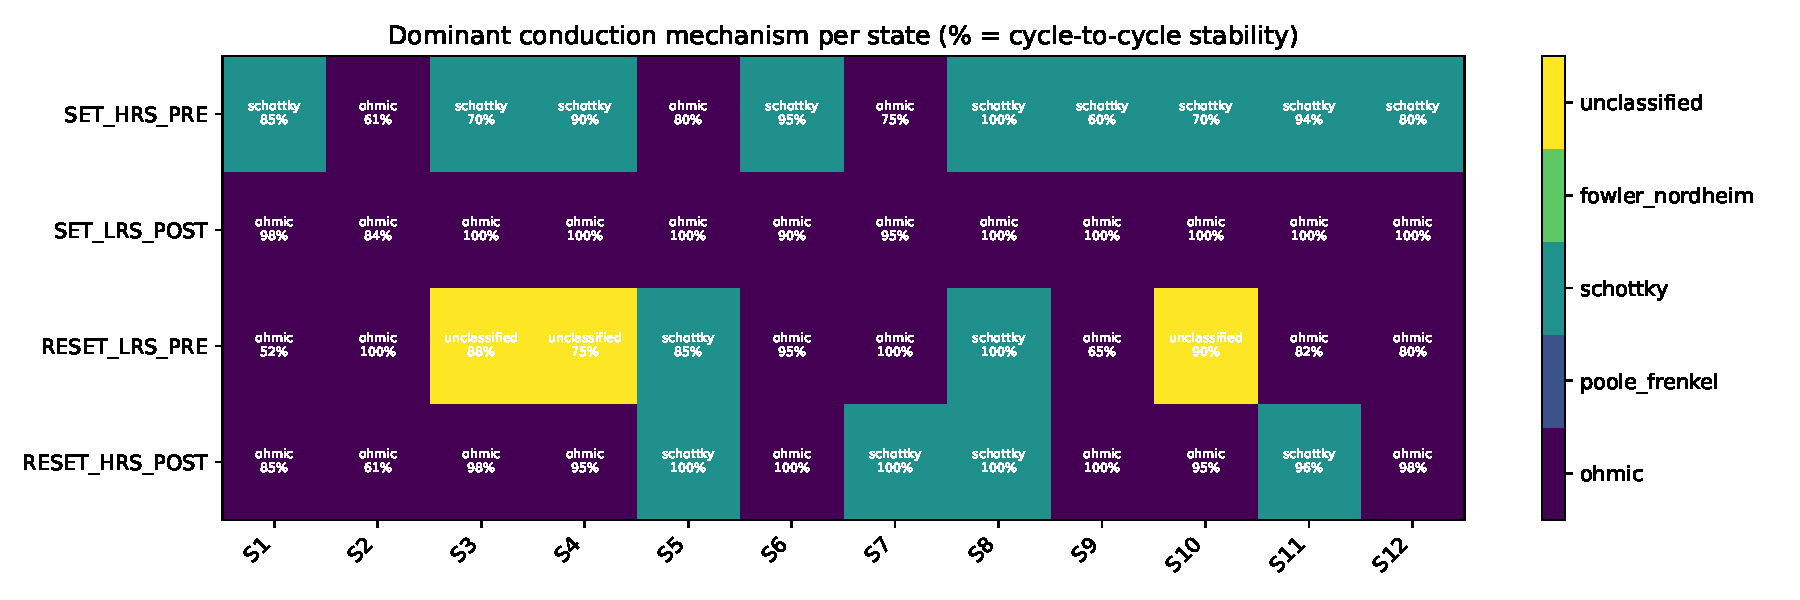
\includegraphics[width=0.98\textwidth]{results/variability/mechanism_map.pdf}
\caption{Dominant conduction mechanism and cycle-to-cycle assignment
stability for each resistance-state segment and deposition condition.  The
post-SET LRS is consistently ohmic, whereas the post-RESET HRS is
Schottky-dominant for all twelve conditions.}
\label{fig:mechanism-map}
\end{figure*}

\subsection{Point-Estimate Fit Quality}
\label{sec:res-fit}

Table~\ref{tab:fitquality} reports unweighted validation RMSE (in decades of
log-current) and Durbin--Watson (DW) statistics for all twelve conditions;
Fig.~\ref{fig:fit-example} shows the S1 overlay and residuals.  SET-branch
RMSE spans 0.47--0.77 decades (mean 0.530) and RESET-branch RMSE spans
0.65--1.02 decades (mean 0.761).  The fitted models capture the hysteresis
ordering, both switching transitions, the compliance plateau, and the LRS
return branches; the dominant residual is a localized error of up to one
decade at the SET transition and along the Schottky-limited HRS approach.

The DW statistics (0.46--1.04, all well below 2) quantify what the overlay
plots suggest: residuals are strongly autocorrelated along the sweep.  We
report this deliberately.  Structured residuals indicate systematic
compact-model mismatch---consistent with the missing interface-conduction
term identified in Section~\ref{sec:res-regimes}---rather than random
measurement noise, and averaging them away with looser metrics would
overstate model adequacy.  S2, with the largest RESET RMSE (1.02 decades)
and the lowest SET DW, also has the least stable Schottky assignment among
the Schottky-dominant pre-SET conditions (60.4\%), supporting this reading.

\begin{table}[!t]
\centering
\caption{Validation fit quality per condition: unweighted RMSE of
$\log_{10}|I|$ (decades) and Durbin--Watson statistics.}
\label{tab:fitquality}
\footnotesize
\begin{tabular}{@{}lcccc@{}}
\toprule
Cond. & RMSE$_{\mathrm{SET}}$ & RMSE$_{\mathrm{RESET}}$ &
DW$_{\mathrm{SET}}$ & DW$_{\mathrm{RESET}}$\\
\midrule
S1  & 0.500 & 0.689 & 0.86 & 0.85\\
S2  & 0.772 & 1.016 & 0.46 & 0.56\\
S3  & 0.566 & 0.659 & 0.72 & 0.98\\
S4  & 0.514 & 0.730 & 0.82 & 0.90\\
S5  & 0.508 & 0.805 & 0.85 & 0.74\\
S6  & 0.468 & 0.650 & 0.94 & 0.93\\
S7  & 0.477 & 0.726 & 1.04 & 0.91\\
S8  & 0.495 & 1.001 & 1.03 & 0.54\\
S9  & 0.510 & 0.700 & 0.92 & 1.04\\
S10 & 0.508 & 0.718 & 1.00 & 0.98\\
S11 & 0.494 & 0.753 & 0.92 & 0.88\\
S12 & 0.548 & 0.681 & 0.96 & 1.01\\
\midrule
Mean & 0.530 & 0.761 & -- & --\\
\bottomrule
\end{tabular}
\end{table}

\begin{figure}[!t]
\centering
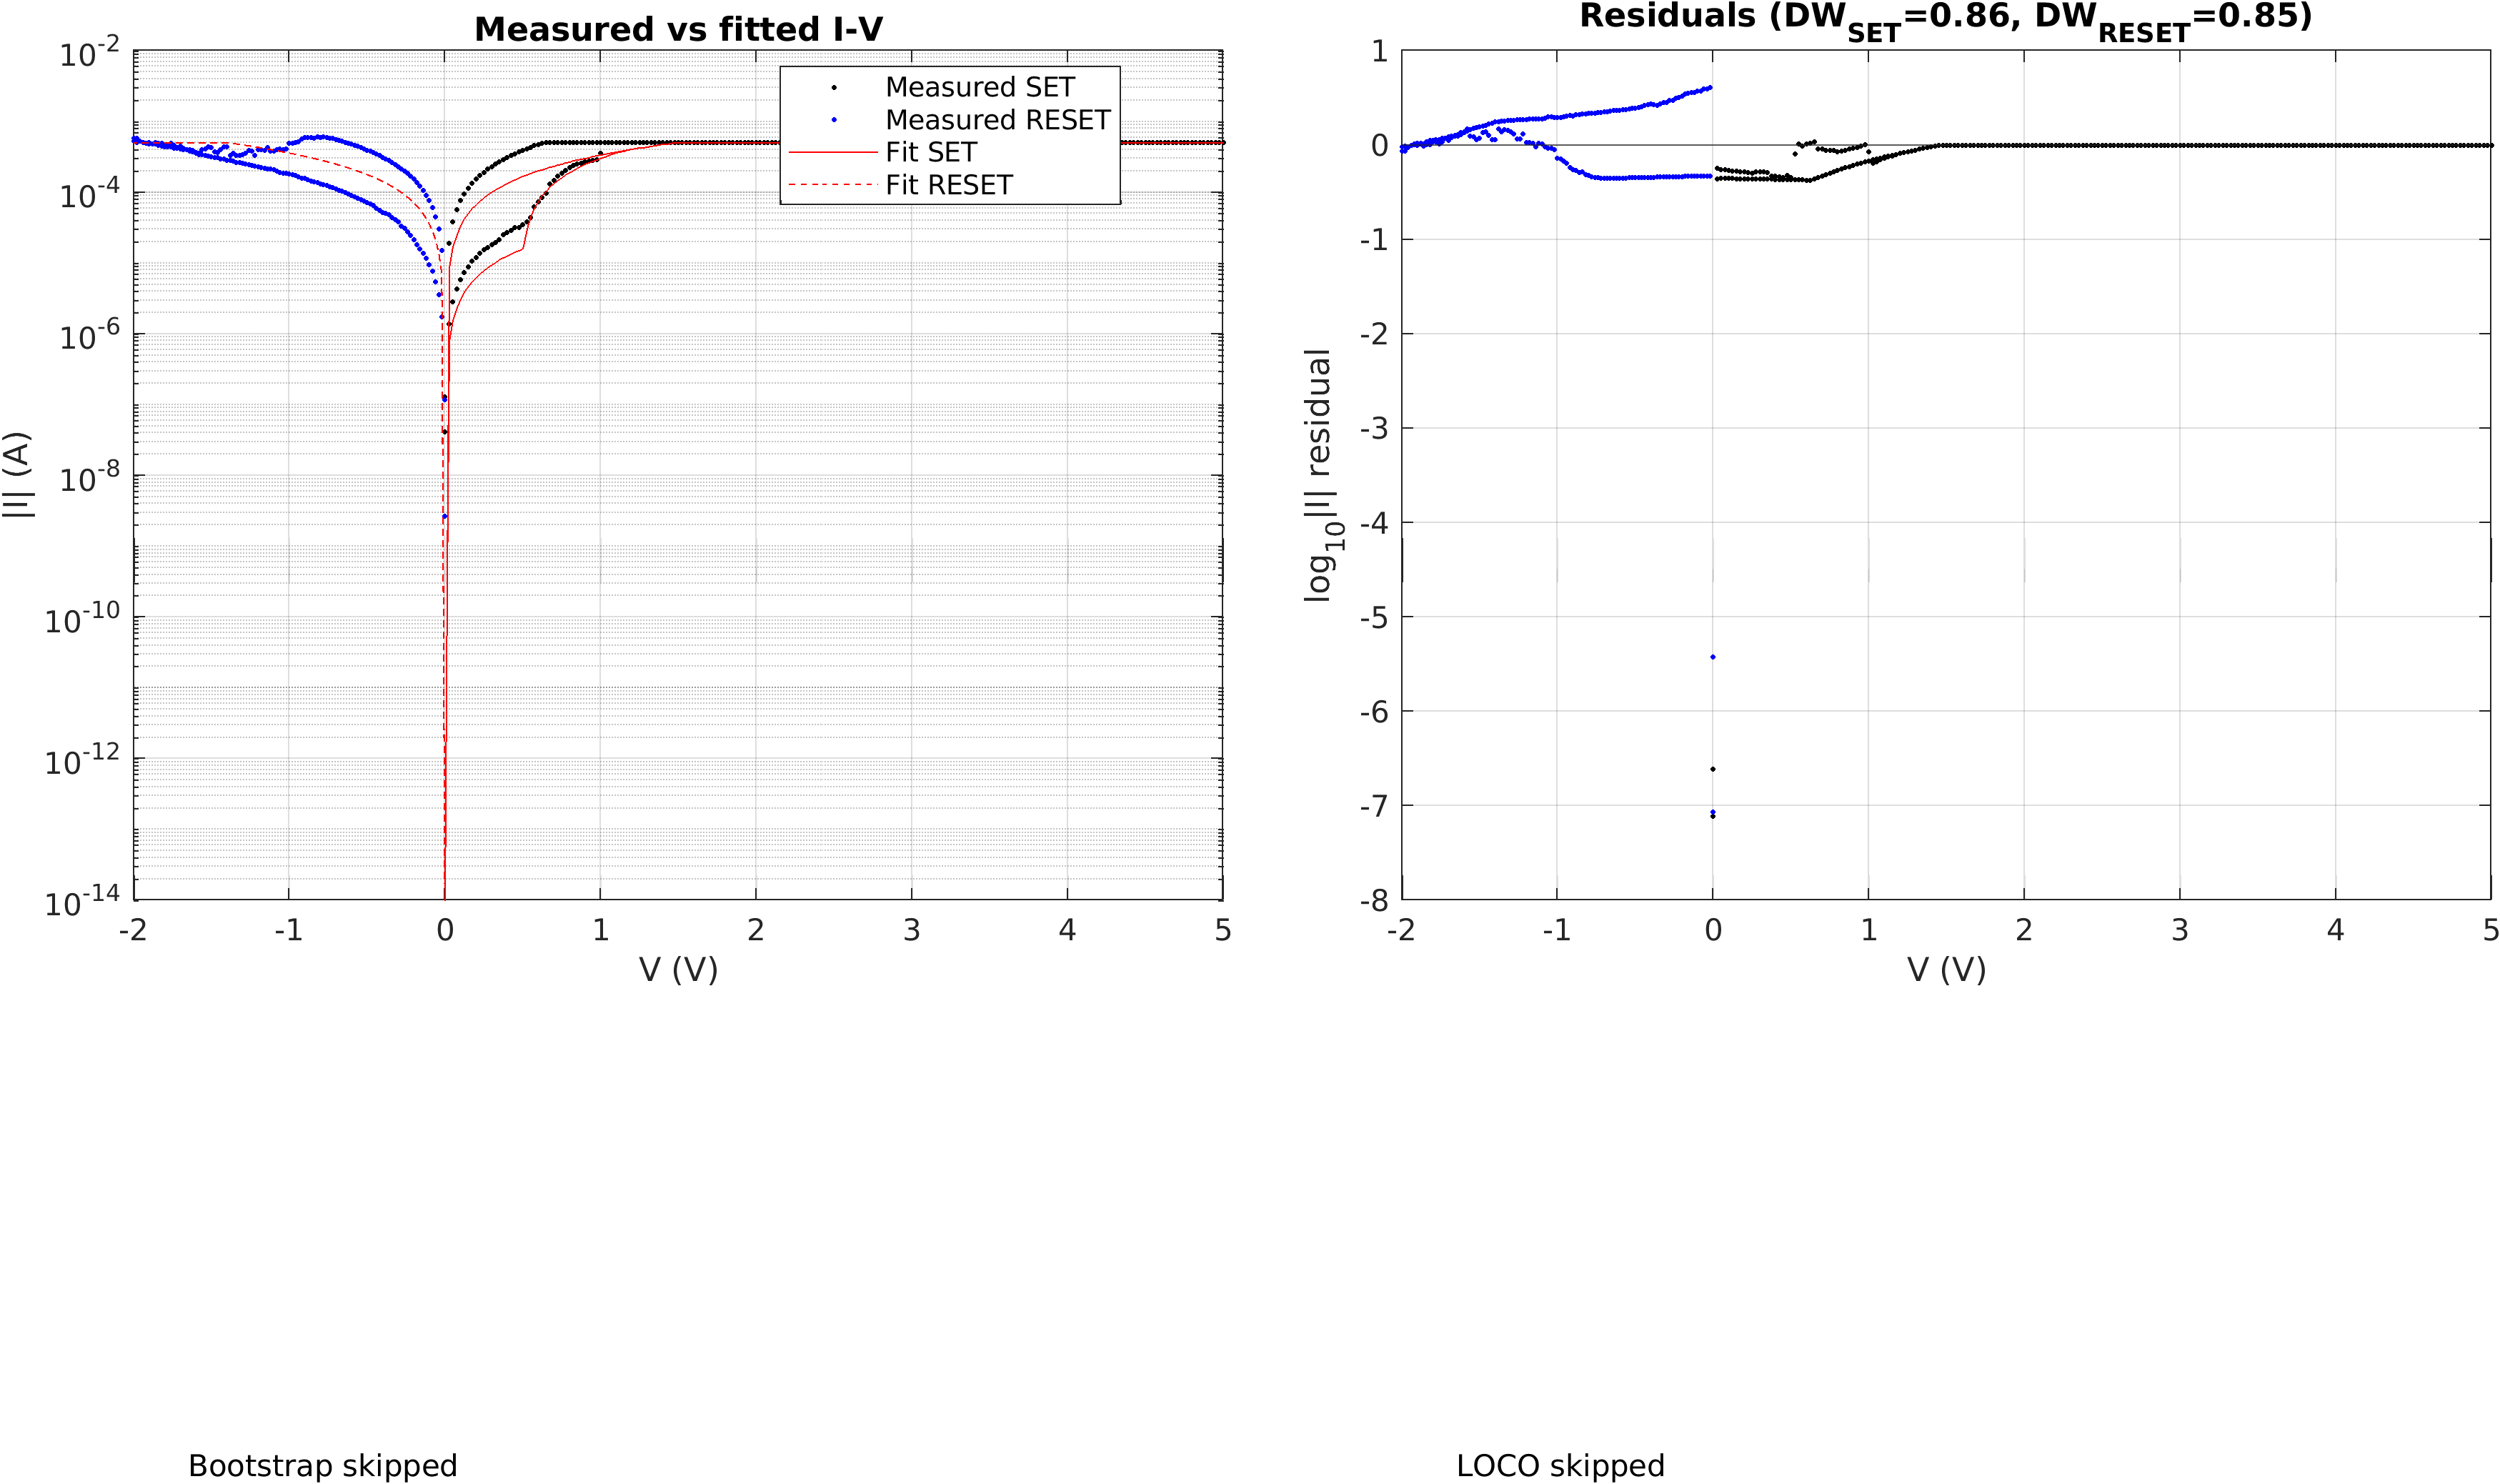
\includegraphics[width=\columnwidth,trim=0 100 0 0,clip]{results/ablation/S1/physics_regime_bo/fit_quality.png}
\caption{Measured versus fitted $I$--$V$ for condition S1 (left) and
log-current residuals along the sweep (right).  The fit reproduces the
butterfly hysteresis, both transitions, and the compliance plateau; the
residual concentrates at the SET transition and the Schottky-limited HRS
approach.}
\label{fig:fit-example}
\end{figure}

\subsection{Identifiability: What DC Data Actually Constrain}
\label{sec:res-ident}

Figure~\ref{fig:ident} shows the Fisher relative-uncertainty heatmap across
all twelve conditions for the archived physics-prior BO point estimates.
This audit uses the same 16-active-parameter model and data as the full
method; the regime-conditioned arm is evaluated separately in the ablation
and bootstrap studies.  Taken at face value, 0--8 of the 16 active
parameters per condition classify as Fisher-identifiable, with a mean of
2.4.  The Fisher condition numbers range from $6.2\times10^{18}$ to
$1.6\times10^{66}$, confirming an extremely sloppy parameterization whose
pseudo-inverse uncertainties must be interpreted cautiously.

Series resistance is the most recurrent nominally identifiable coordinate
(8 of 12 conditions), followed by $F_{\min,\mathrm{RESET}}$ (5 of 12) and
$V_{0,\mathrm{SET}}$, $V_{0,\mathrm{RESET}}$, and
$F_{\min,\mathrm{SET}}$ (4 of 12 each).  Neither $I_0$ nor $g_0$, and none
of the four fitted gap-limit/initialization parameters, is Fisher-identifiable
on any condition.  Isolated identifiable classifications for activation
energy or velocity prefactor occur only on S9 or S12 and are not stable
across the replicated center-point conditions S9--S12.  Extremely small
pseudo-inverse uncertainties on individual $F_{\min}$ entries are therefore
treated as local numerical results, not as proof of global uniqueness.

The defensible interpretation is that DC butterfly data constrain effective
branch scales---series resistance, voltage curvature, and switching-field
combinations---more reliably than the decomposition into $I_0$, $g_0$,
activation energies, velocity prefactors, and gap geometry.  The bootstrap
results in Section~\ref{sec:res-variability} independently reinforce this
conclusion by showing substantial parameter movement under resampling of the
measured cycles.

\begin{figure}[!t]
\centering
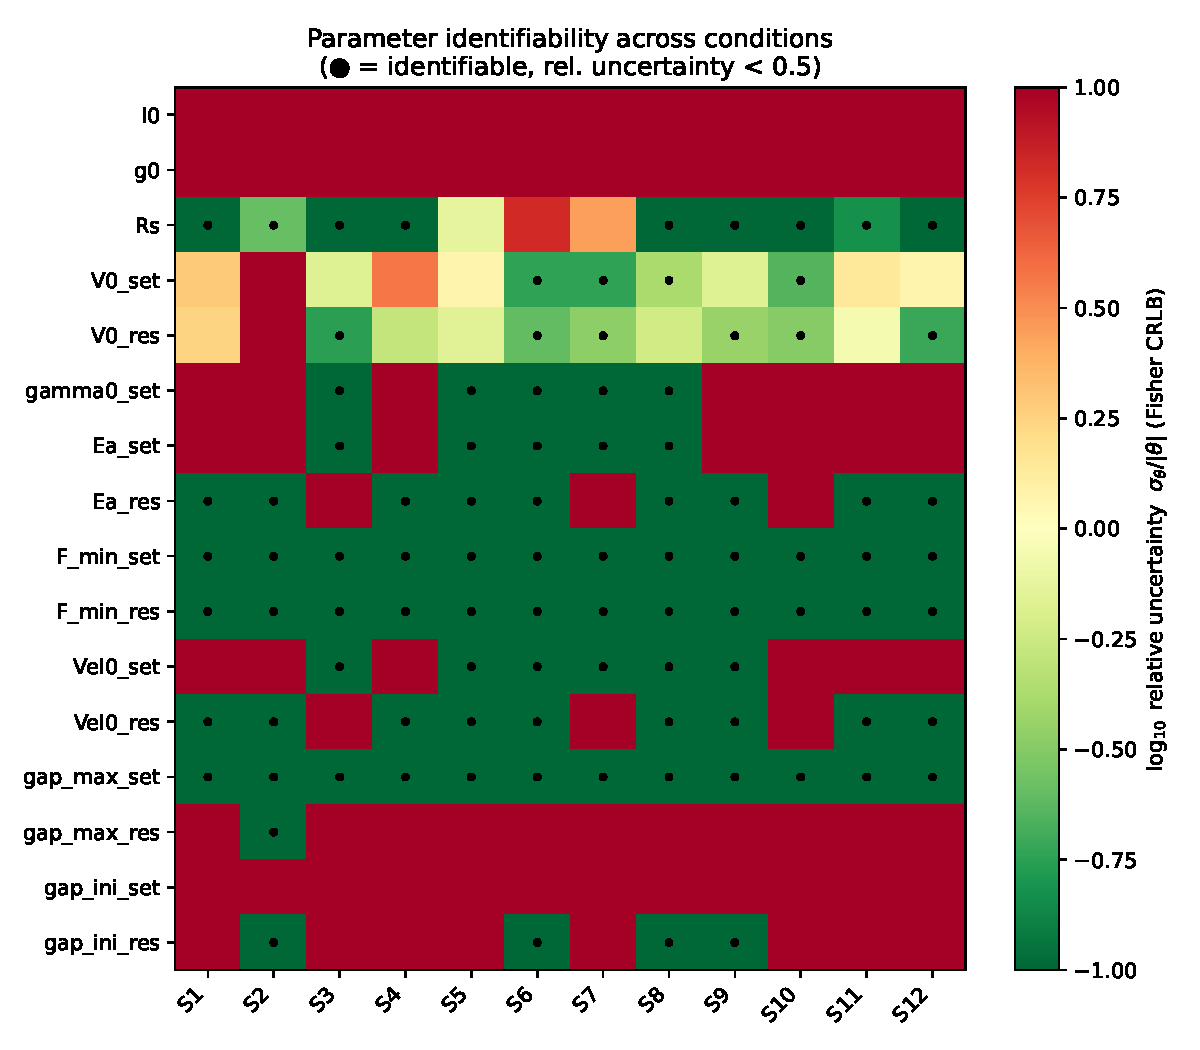
\includegraphics[width=\columnwidth]{results/publication/identifiability_heatmap.pdf}
\caption{Fisher relative uncertainty $\sigma_\theta/|\theta|$ (log color
scale) for the 16 active Stanford parameters across the twelve conditions;
dots mark the nominal identifiable class ($\rho<0.5$).  The very large
condition numbers require these local classifications to be interpreted
together with cycle-bootstrap stability.}
\label{fig:ident}
\end{figure}

\subsection{Ablation: What Each Ingredient Buys}
\label{sec:res-ablation}

Table~\ref{tab:ablation} compares the extraction variants on unweighted
validation RMSE averaged over all twelve conditions.  Bayesian optimization
is decisive on RESET: physics-informed prior means without optimization
(\texttt{physics\_nobo}) yield $1.528\pm0.434$ decades, versus
$0.756\pm0.124$ with BO.  SET is less sensitive because its LRS and
compliance-limited portions are already close to the prior prediction.

The three optimized variants have nearly identical aggregate unweighted
error.  The full regime-aware method gives 0.530/0.761 decades, legacy
physics priors give 0.546/0.756, and uninformative priors give 0.537/0.755.
Thus, regime conditioning and informative priors should not be sold as an
RMSE improvement.  Their role is to prevent unsupported Schottky/FN windows
from steering a bulk-current model and to document how poorly identified
coordinates are selected.  In a sloppy model, comparable errors from
different prior structures are themselves evidence that an overlay is
insufficient to establish physical parameter extraction.

\begin{table}[!t]
\centering
\caption{Ablation over all 12 conditions: unweighted validation RMSE
(decades), mean $\pm$ standard deviation across conditions.}
\label{tab:ablation}
\footnotesize
\begin{tabular}{@{}lcc@{}}
\toprule
Variant & RMSE$_{\mathrm{SET}}$ & RMSE$_{\mathrm{RESET}}$\\
\midrule
Regime-conditioned + weighting & $0.530\pm0.081$ & $0.761\pm0.123$\\
Physics priors + BO & $0.546\pm0.077$ & $0.756\pm0.124$\\
Uninformative priors + BO & $0.537\pm0.076$ & $0.755\pm0.126$\\
Physics priors, no BO & $0.571\pm0.115$ & $1.528\pm0.434$\\
\bottomrule
\end{tabular}
\end{table}

\subsection{Cycle-to-Cycle Variability}
\label{sec:res-variability}

The cluster bootstrap of Section~\ref{sec:boot} propagates cycle-to-cycle
variability of the selected device into empirical 95\% intervals for every
active parameter.  All 2400 refits (200 draws for each of 12 conditions)
completed, and all 192 condition--parameter intervals are finite and
nondegenerate.  Figure~\ref{fig:param-cv} reports the coefficient of
variation (CV) of each bootstrap distribution.  The median CV over all
entries is 0.448, with a range of 0.202--2.698.

The largest cross-cycle instability occurs in $R_s$ (median CV 1.444) and
the SET/RESET velocity prefactors (1.194 and 1.282).  Current scale $I_0$
and activation energies also vary substantially (median CV 0.566 and
0.456--0.591).  The branch voltage scales are more repeatable, with median
CV near 0.28, consistent with the switching-curve shape directly constraining
them.  Some gap parameters show lower CV despite failing the Fisher test;
this is not contradictory because a bounded, prior-centered optimizer can
return a stable coordinate even when the likelihood supplies little local
information.  Bootstrap repeatability and identifiability therefore answer
different questions and must be reported together.

\begin{figure}[!t]
\centering
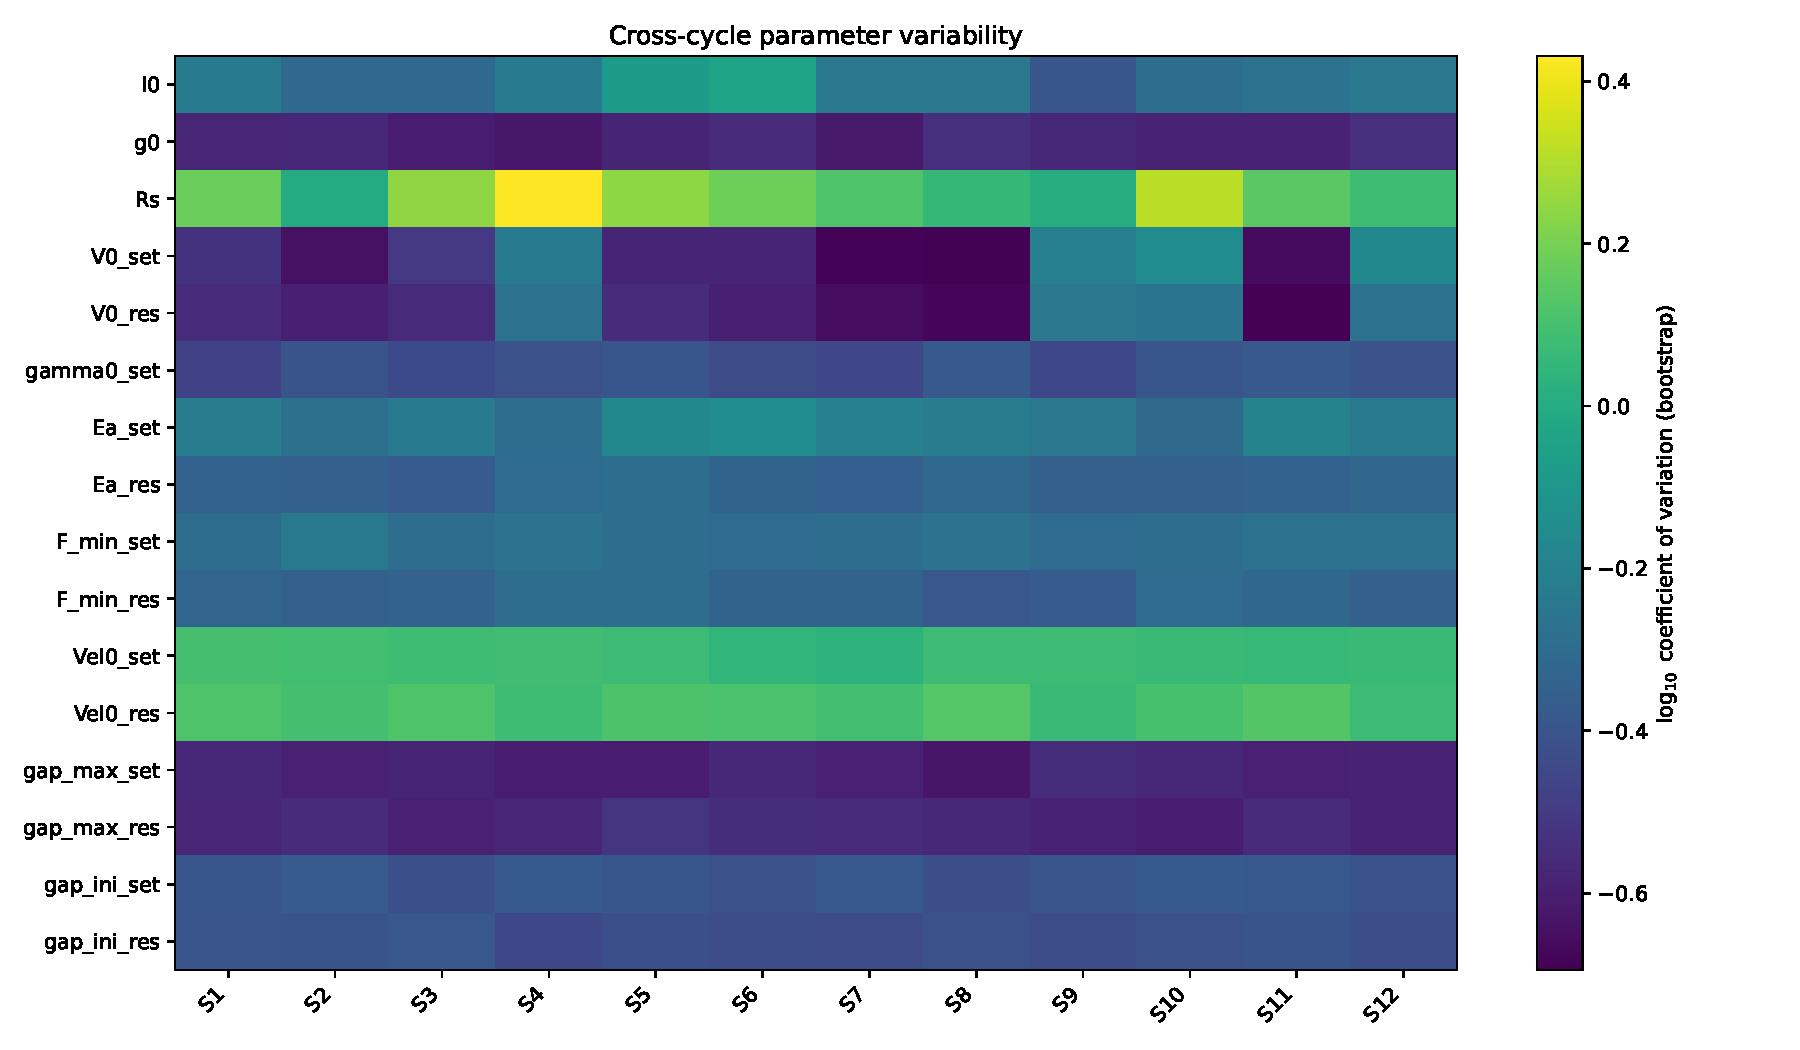
\includegraphics[width=\columnwidth]{results/variability/parameter_cv.pdf}
\caption{Cycle-to-cycle parameter variability from 200 cluster-bootstrap
refits per condition.  Color denotes $\log_{10}(\mathrm{CV})$.  Series
resistance and velocity prefactors are the least stable, while the branch
voltage scales are comparatively repeatable.}
\label{fig:param-cv}
\end{figure}

% =========================================================================
\section{Discussion}
\label{sec:discussion}
% =========================================================================

\subsection{Implications for Compact-Model Users}

For circuit designers consuming calibrated Stanford parameter sets, the
practical messages are direct.  (i)~Treat per-condition parameter files as
\emph{behavioral} calibrations valid for the fitted protocol; only the
identifiable combinations transfer with evidential support.  (ii)~Do not
ascribe physical meaning to fitted $E_a$, $\nu_0$, or gap geometry obtained
from DC sweeps alone; constraining kinetics requires pulsed or
sweep-rate-resolved data, which break the quasi-static degeneracy between
kinetic prefactors and the time axis.  (iii)~When comparing parameters
across deposition conditions (the response-surface use case of
Table~\ref{tab:doe}), compare identifiable combinations---LRS resistance
scale, switching thresholds---rather than raw parameter columns, since the
latter mix data- and prior-driven coordinates.

\subsection{Model Adequacy for TaO$_x$}

The regime analysis localizes the Stanford model's structural limitation for
these devices: HRS conduction is interface-limited (Schottky) in nearly all
cycles, while the model's single $\sinh$ current law is bulk-like.  This
mismatch, not optimizer failure, sets the residual floor of
Table~\ref{tab:fitquality}---the three optimized ablation arms have nearly
identical aggregate unweighted RMSE despite different priors and loss
weighting.  A principled
extension would add a barrier-limited HRS current branch (or a
gap-dependent barrier term); the regime map produced here provides exactly
the windows and slopes such an extension should target.  Until then,
down-weighting unmodelable windows during fitting, as done here, prevents
interface physics from contaminating bulk parameters while keeping the
mismatch visible in unweighted validation.

\subsection{Limitations}

The transient replay is quasi-static, so kinetic parameters absorb the
effective time scale.  Fisher analysis is local, and the present result
archive does not contain completed profile-likelihood scans; identifiability
claims are therefore limited to the combined Fisher and bootstrap evidence.
The Fisher audit and full regime-conditioned bootstrap were also archived as
separate runs, so a future release should repeat both diagnostics at one
common optimum.  Bootstrap intervals are cycle-level for one selected device
per condition and do not constitute device-to-device or wafer-level
statistics.  Finally, the reset-side $\gamma_0$ is structurally overridden
under negative bias in the released Verilog-A, so it is retained for model
compatibility but not physically interpreted.

% =========================================================================
\section{Conclusion}
\label{sec:conclusion}
% =========================================================================

We presented a physics-guided, identifiability-aware pipeline that fits the
Stanford RRAM compact model to measured TaO$_x$ DC switching data and
reports, with every parameter set, the evidence behind it.  Applied
uniformly to twelve sputter-deposition conditions, the flow achieves
mean RMSE of 0.530 decades for SET and 0.761 decades for RESET while
establishing three findings that overlay plots alone cannot.  First, only
0--8 of 16 active parameters per condition pass the local Fisher threshold,
and the matrices remain extremely ill-conditioned.  Second, 200 cycle-level
bootstrap refits per condition reveal substantial parameter variability,
particularly in series resistance and velocity prefactors.  Third, the
post-RESET HRS is Schottky-dominant in 92.5--100\% of cycles for every
condition, a mechanism outside the Stanford bulk current law that bounds
achievable fit fidelity.  Fit quality, regime validity, identifiability, and
cycle-level uncertainty should therefore be reported together as the
deliverable of RRAM compact-model calibration.

% =========================================================================
\begin{thebibliography}{12}\footnotesize

\bibitem{wong2012metal}
H.-S.~P. Wong \emph{et~al.}, ``Metal-oxide RRAM,'' \emph{Proc. IEEE},
vol.~100, no.~6, pp. 1951--1970, Jun. 2012.

\bibitem{ielmini2018inmemory}
D.~Ielmini and H.-S.~P. Wong, ``In-memory computing with resistive switching
devices,'' \emph{Nature Electron.}, vol.~1, pp. 333--343, 2018.

\bibitem{guan2012spice}
X.~Guan, S.~Yu, and H.-S.~P. Wong, ``A SPICE compact model of metal oxide
resistive switching memory with variations,'' \emph{IEEE Electron Device
Lett.}, vol.~33, no.~10, pp. 1405--1407, Oct. 2012.

\bibitem{jiang2016verification}
Z.~Jiang \emph{et~al.}, ``A compact model for metal--oxide resistive random
access memory with experiment verification,'' \emph{IEEE Trans. Electron
Devices}, vol.~63, no.~5, pp. 1884--1892, May 2016.

\bibitem{transtrum2015sloppiness}
M.~K. Transtrum, B.~B. Machta, K.~S. Brown, B.~C. Daniels, C.~R. Myers, and
J.~P. Sethna, ``Perspective: Sloppiness and emergent theories in physics,
biology, and beyond,'' \emph{J. Chem. Phys.}, vol. 143, no.~1, Art. no.
010901, 2015.

\bibitem{chowdhury2025mwscas}
M.~T.~R. Chowdhury, A.~Moazzeni, and G.~Tutuncuoglu, ``Atomic-scale insights
into the switching mechanisms of RRAM devices,'' in \emph{Proc. IEEE 68th
Int. Midwest Symp. Circuits Syst. (MWSCAS)}, Lansing, MI, USA, 2025,
pp. 518--522.

\bibitem{moazzeni2023}
A.~Moazzeni, M.~T.~R. Chowdhury, and G.~Tutuncuoglu, ``The impact of
operation conditions on potentiation, depression and endurance dynamics of
tantalum oxide RRAMs,'' in \emph{Proc. IEEE Int. Integr. Rel. Workshop
(IIRW)}, 2023.

\bibitem{chiu2014}
F.-C. Chiu, ``A review on conduction mechanisms in dielectric films,''
\emph{Adv. Mater. Sci. Eng.}, vol. 2014, Art. no. 578168, 2014.

\bibitem{raue2009}
A.~Raue \emph{et~al.}, ``Structural and practical identifiability analysis
of partially observed dynamical models by exploiting the profile
likelihood,'' \emph{Bioinformatics}, vol.~25, no.~15, pp. 1923--1929, 2009.

\bibitem{snoek2012practical}
J.~Snoek, H.~Larochelle, and R.~P. Adams, ``Practical Bayesian optimization
of machine learning algorithms,'' in \emph{Proc. Adv. Neural Inf. Process.
Syst. (NeurIPS)}, 2012, pp. 2951--2959.

\bibitem{lee2011fast}
M.-J. Lee \emph{et~al.}, ``A fast, high-endurance and scalable non-volatile
memory device made from asymmetric Ta$_2$O$_{5-x}$/TaO$_{2-x}$ bilayer
structures,'' \emph{Nature Mater.}, vol.~10, pp. 625--630, 2011.

\end{thebibliography}

\end{document}
